\documentclass{beamer}
% \usepackage[brazil]{babel}
\usepackage[utf8]{inputenc}
\usepackage{fancybox}
\title[Research]{Research}
%\subtitle[short version]{}
%\date{}
\author[Sivaram Ambikasaran]{Sivaram Ambikasaran}
\institute[IITM]{Indian Institute of Technology Madras}
\usetheme{Madrid}

\newcommand{\dsum}{\displaystyle\sum}
\newcommand{\magn}[1]{\left\lVert#1\right\rVert}
\newcommand{\Rb}{\mathbb{R}}



\usecolortheme{owl}
\setbeamercolor{normal text}{fg=orange}
\usebeamercolor*{normal text}
\begin{document}
\frame{\titlepage}

\begin{frame}{Who are we?}
	
\includegraphics[width=\textwidth]{./images/SAFRAN_Logo.png}
	\begin{center}
	Stable Accurate Fast Robust Algorithms \& Numerics group
	\end{center}
\end{frame}

\begin{frame}{Who are we?}
	\begin{center}
	\huge{Current students}
	\end{center}
	\includegraphics[width=0.2\textwidth]{./images/Kandappan.jpg} \hspace{1em}
	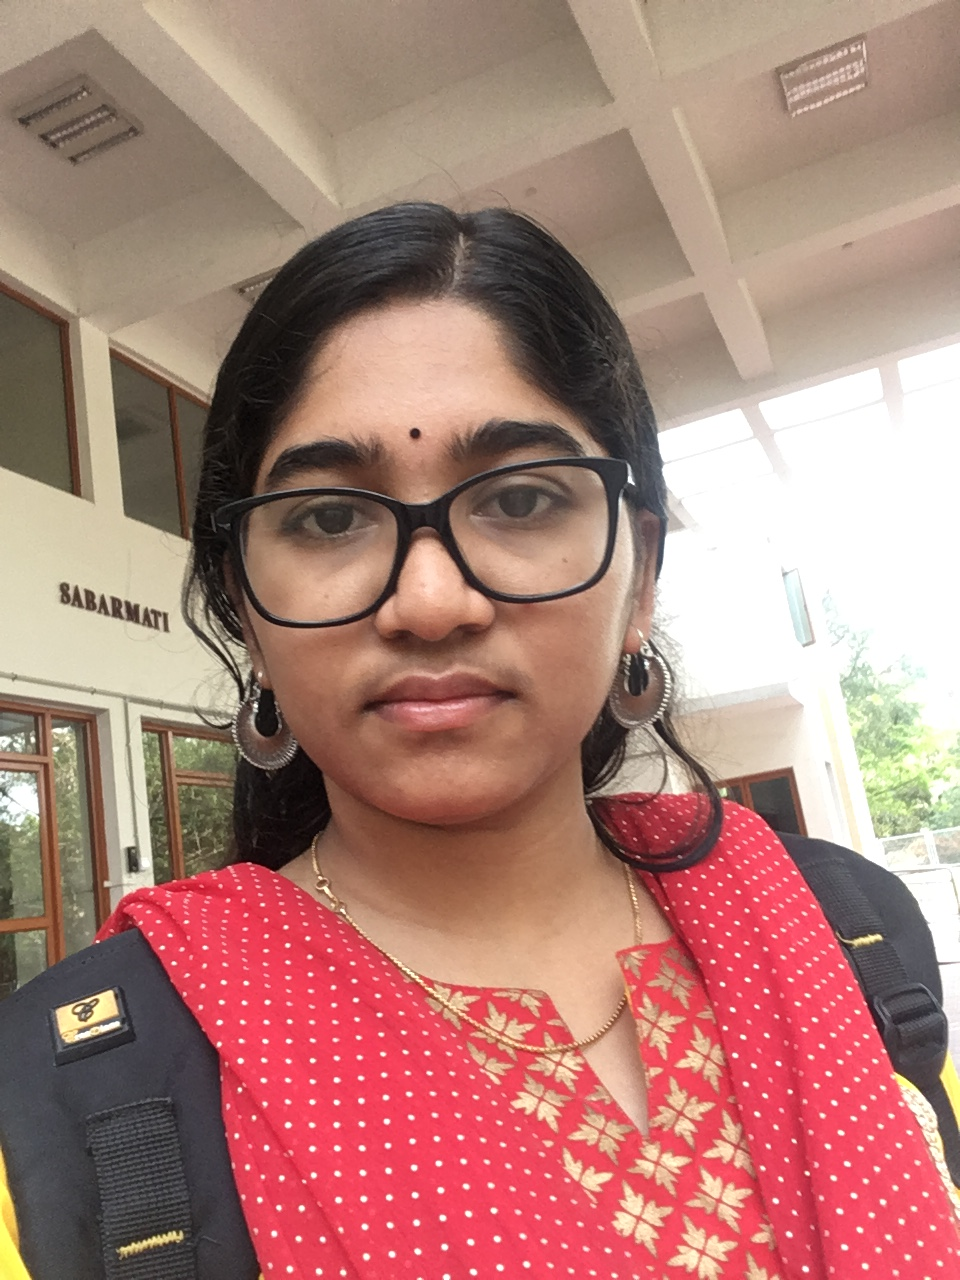
\includegraphics[width=0.2\textwidth]{./images/Vaishnavi.jpeg} \hspace{1em}
	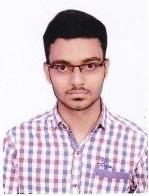
\includegraphics[width=0.2025\textwidth]{./images/Ritesh.jpg} \hspace{1em}
	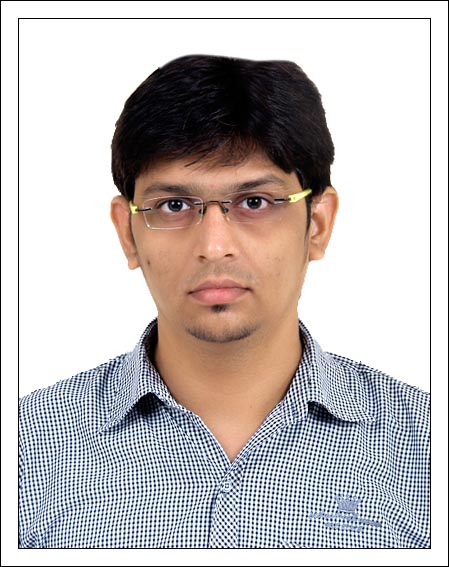
\includegraphics[width=0.21\textwidth]{./images/Pragnesh.jpg}
\end{frame}

\begin{frame}{Who are we?}
	\begin{center}
	\huge{Alumni}
	\end{center}
	\begin{center}
	\includegraphics[width=0.2\textwidth]{./images/Shyam.jpeg} \hspace{1em}
	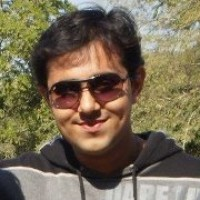
\includegraphics[width=0.2\textwidth]{./images/Karan.jpeg} \hspace{1em}
	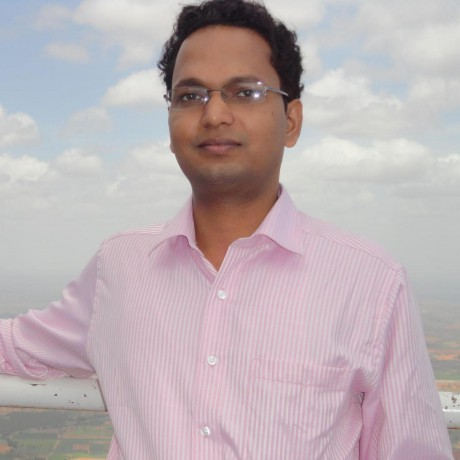
\includegraphics[width=0.2025\textwidth]{./images/Nachiketa.jpg} \hspace{1em}
	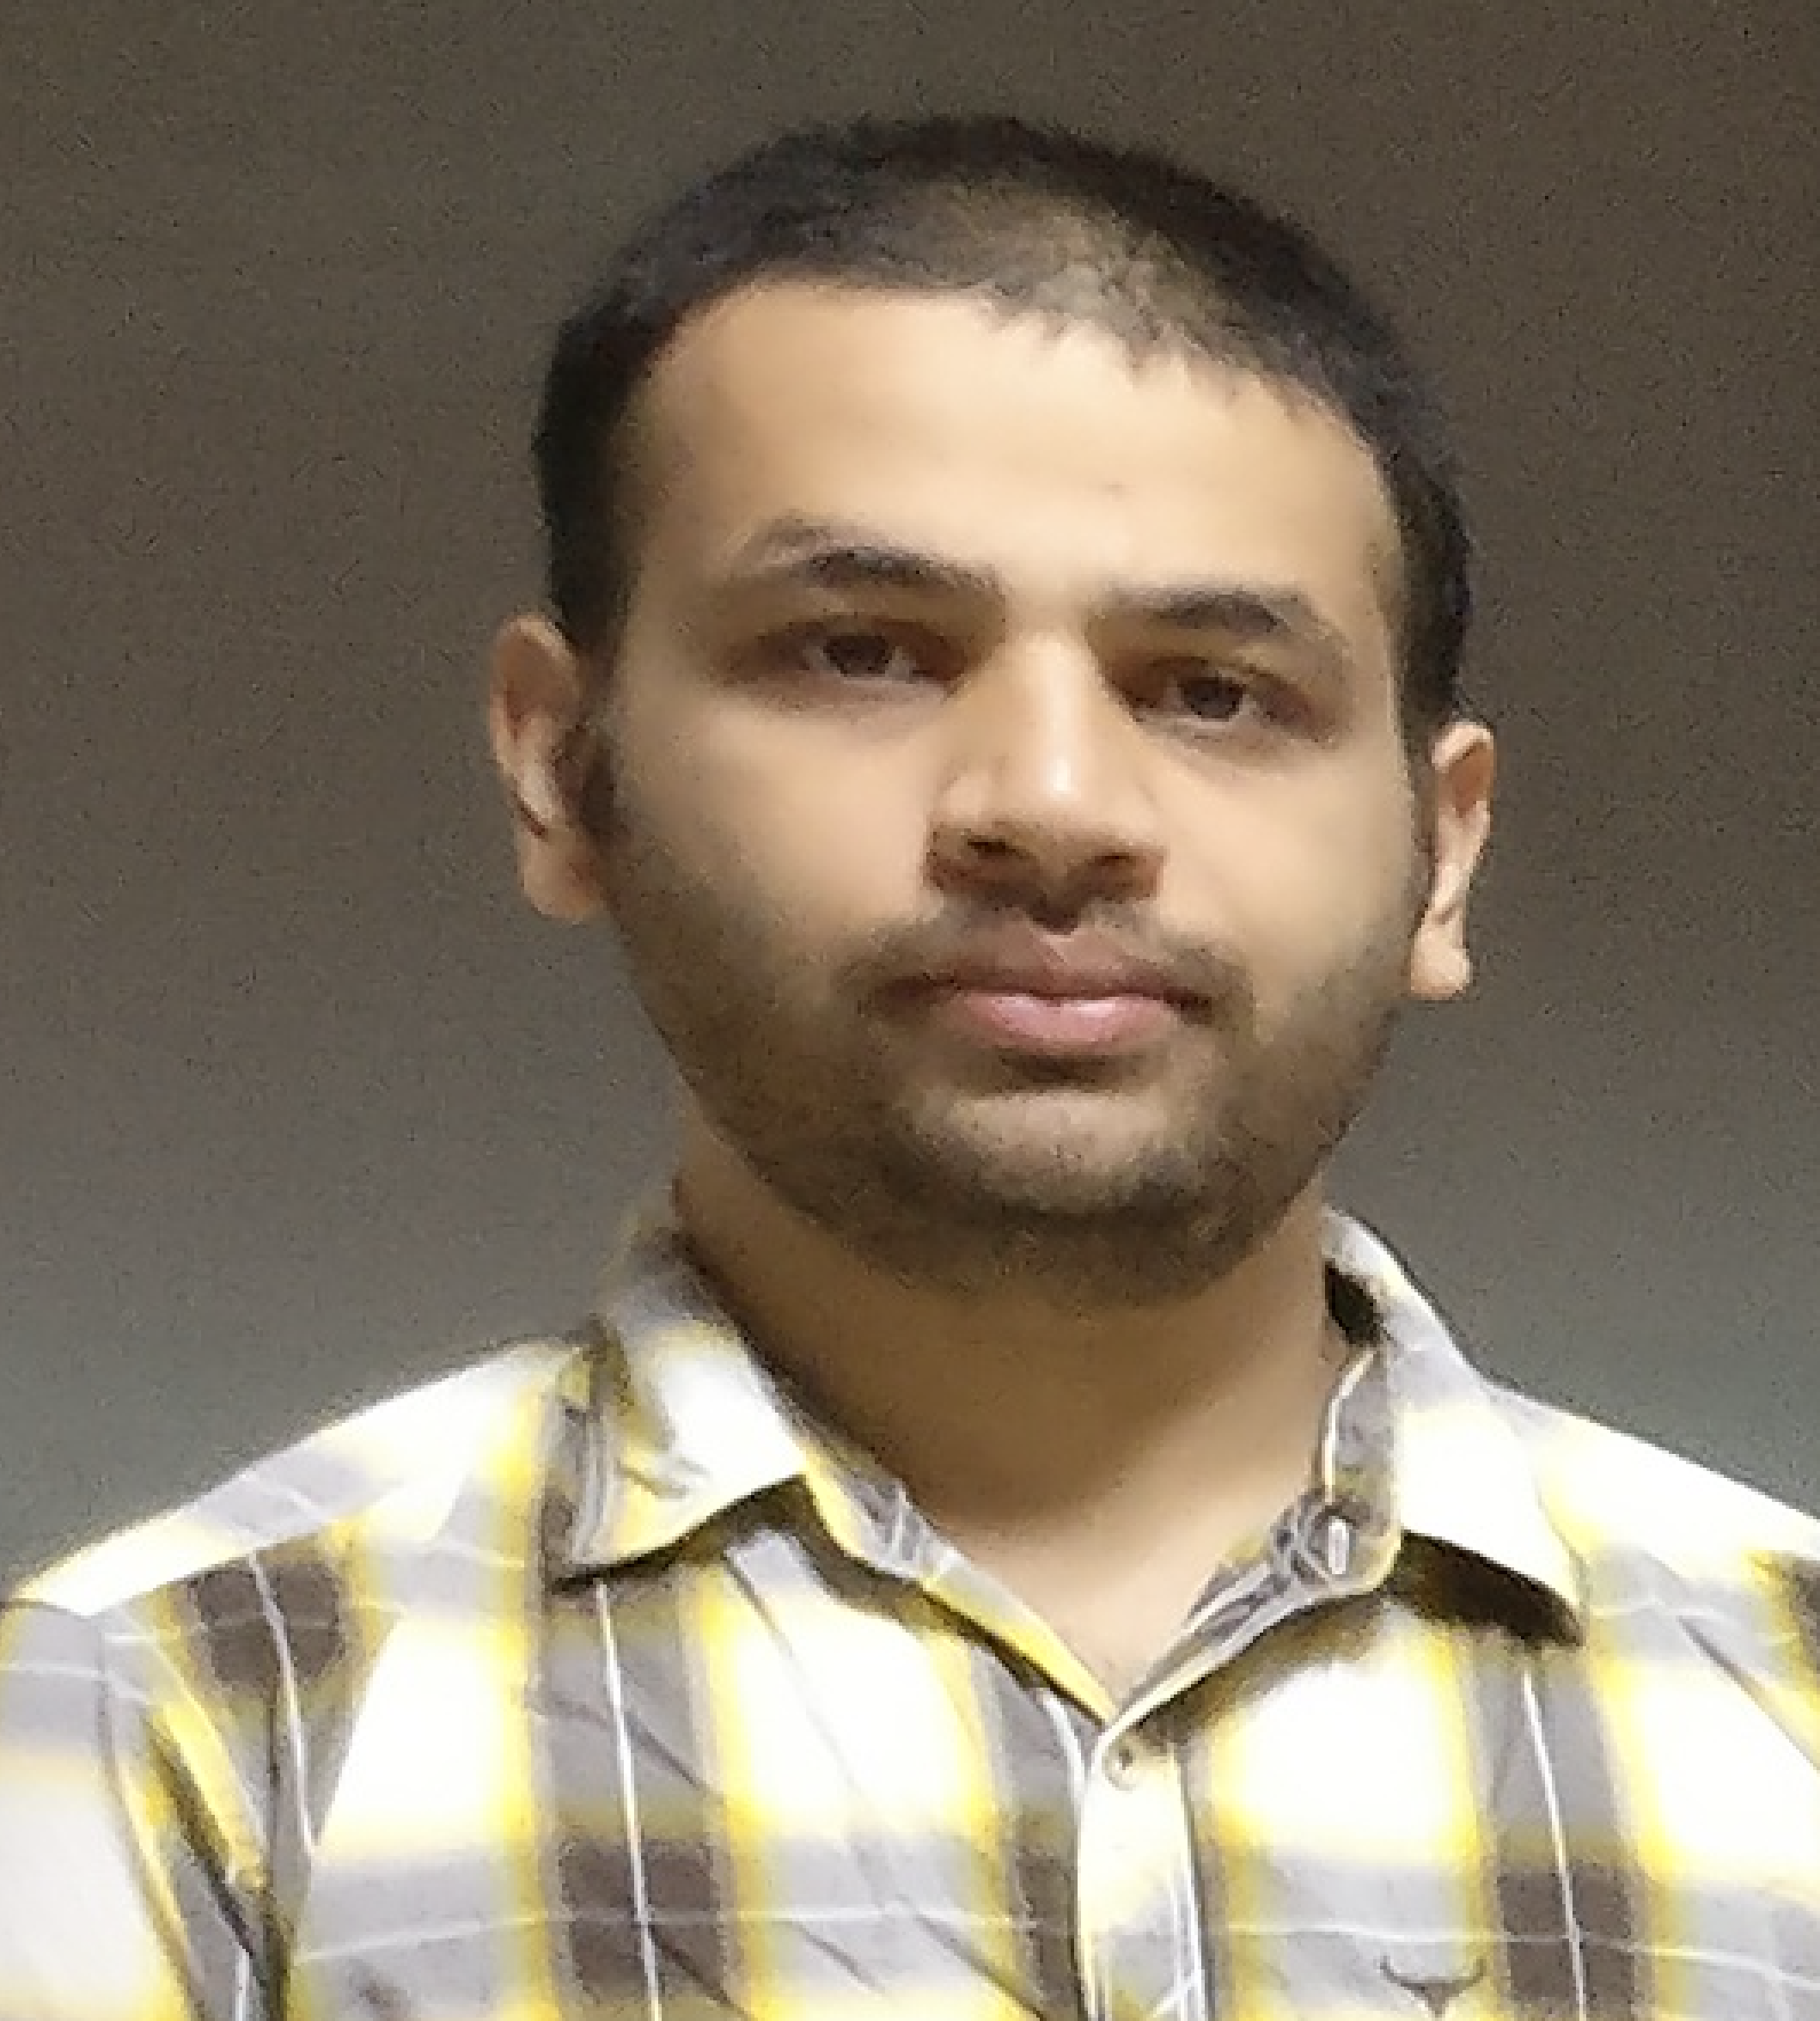
\includegraphics[width=0.2025\textwidth]{./images/Abhay.png} \hspace{1em}
	\end{center}
\end{frame}

\begin{frame}{What to we do?}
	\Large
	\begin{center}
	Design and construct highly accurate fast matrix algorithms
	\begin{itemize}
		\item
		Accurate - User prescribes the accuracy he wants
		\item
		Fast - Scales linearly with problem size
	\end{itemize}
	\end{center}
\end{frame}

\begin{frame}{Why do we do?}
	\begin{itemize}
		\item
		Matrix computations form the backbone of computational science
		\item
		Need to develop novel matrix algorithms that can scale up to handle these large problems
		\item
		Today’s applications involve large matrices and massive data sets
		\begin{itemize}
			\item
			Finite element/ Integral equation solvers for scattering applications
			\item
			Data driven physical modelling
			\item
			High dimensional statistics
		\end{itemize}
	\end{itemize}
\end{frame}

\begin{frame}{How do we achieve our goals?}
	\begin{itemize}
		\item
		Leverage tools from approximation theory and numerical linear algebra
		\item
		Guaranteed error bounds for all the algorithms
	\end{itemize}
\end{frame}

\begin{frame}{Example: Computational Physics}
	\begin{itemize}
		\item
		$N$ charges: $\{q_i,r_i\}_{i=1}^N$
		\item
		Potential: $\phi_i = \dsum_{j \neq i} \dfrac{q_j}{\magn{r_i-r_j}}$ for $i \in \{1,2,\ldots,N\}$
		\item
		Note that we have $\phi = Aq$, $\phi$ is the set of potentials, $q$ is the set of charges and $A_{ij} = \dfrac1{\magn{r_i-r_j}}$ for $i \neq j$
		\item
		Matrix-vector product: Given $q$, compute $\phi$. Cost is $\mathcal{O}(N^2)$
		\item
		Solve linear system: Given $\phi$, compute $q$. Cost is $\mathcal{O}(N^3)$
		\item
		Can we reduce the above computational complexity to say $\mathcal{O}_{\epsilon}(N)$?
	\end{itemize}
\end{frame}

\begin{frame}{Example: High dimensional statistics}
	\begin{itemize}
		\item
		Given a covariance matrix $\Sigma \in \Rb^{N \times N}$, can we efficiently generate samples possessing the desired covariance structure?
		\item
		Naive way is to compute the Cholesky decomposition of $\Sigma$, which costs $\mathcal{O}(N^3)$.
		\item
		Can we reduce the computational complexity to $\mathcal{O}_{\epsilon}(N)$?
	\end{itemize}
\end{frame}

\begin{frame}
	\begin{itemize}
		\item
		Turns out we can reduce the above complexities to $\mathcal{O}(N)$ in both the above problem
		\item
		Leveraging the fact that the matrices that show up have a hierarchical low-rank structure
		\item
		Enables compression of sub-blocks of matrices and thereby reducing the complexity
	\end{itemize}
\end{frame}

\begin{frame}{HODLR}
	\begin{center}
	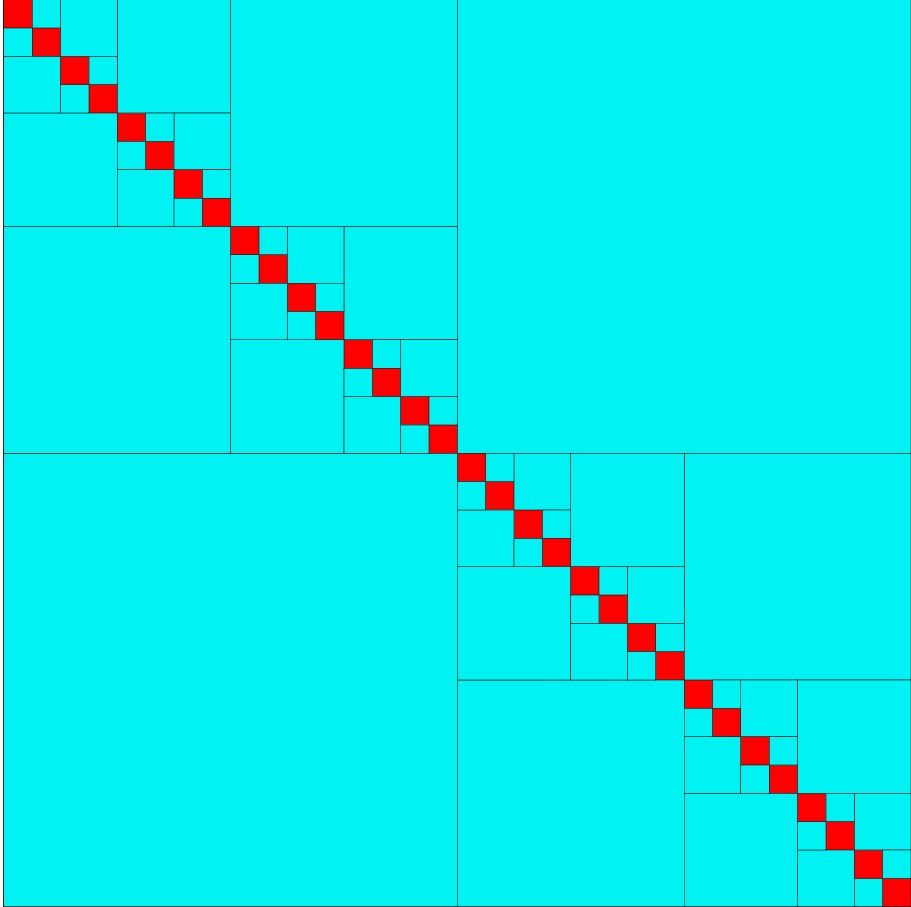
\includegraphics[width=0.5\textwidth]{./images/HSS_level_5.jpg}
	\end{center}
\end{frame}

\begin{frame}{$\mathcal{H}$-matrix}
	\begin{center}
	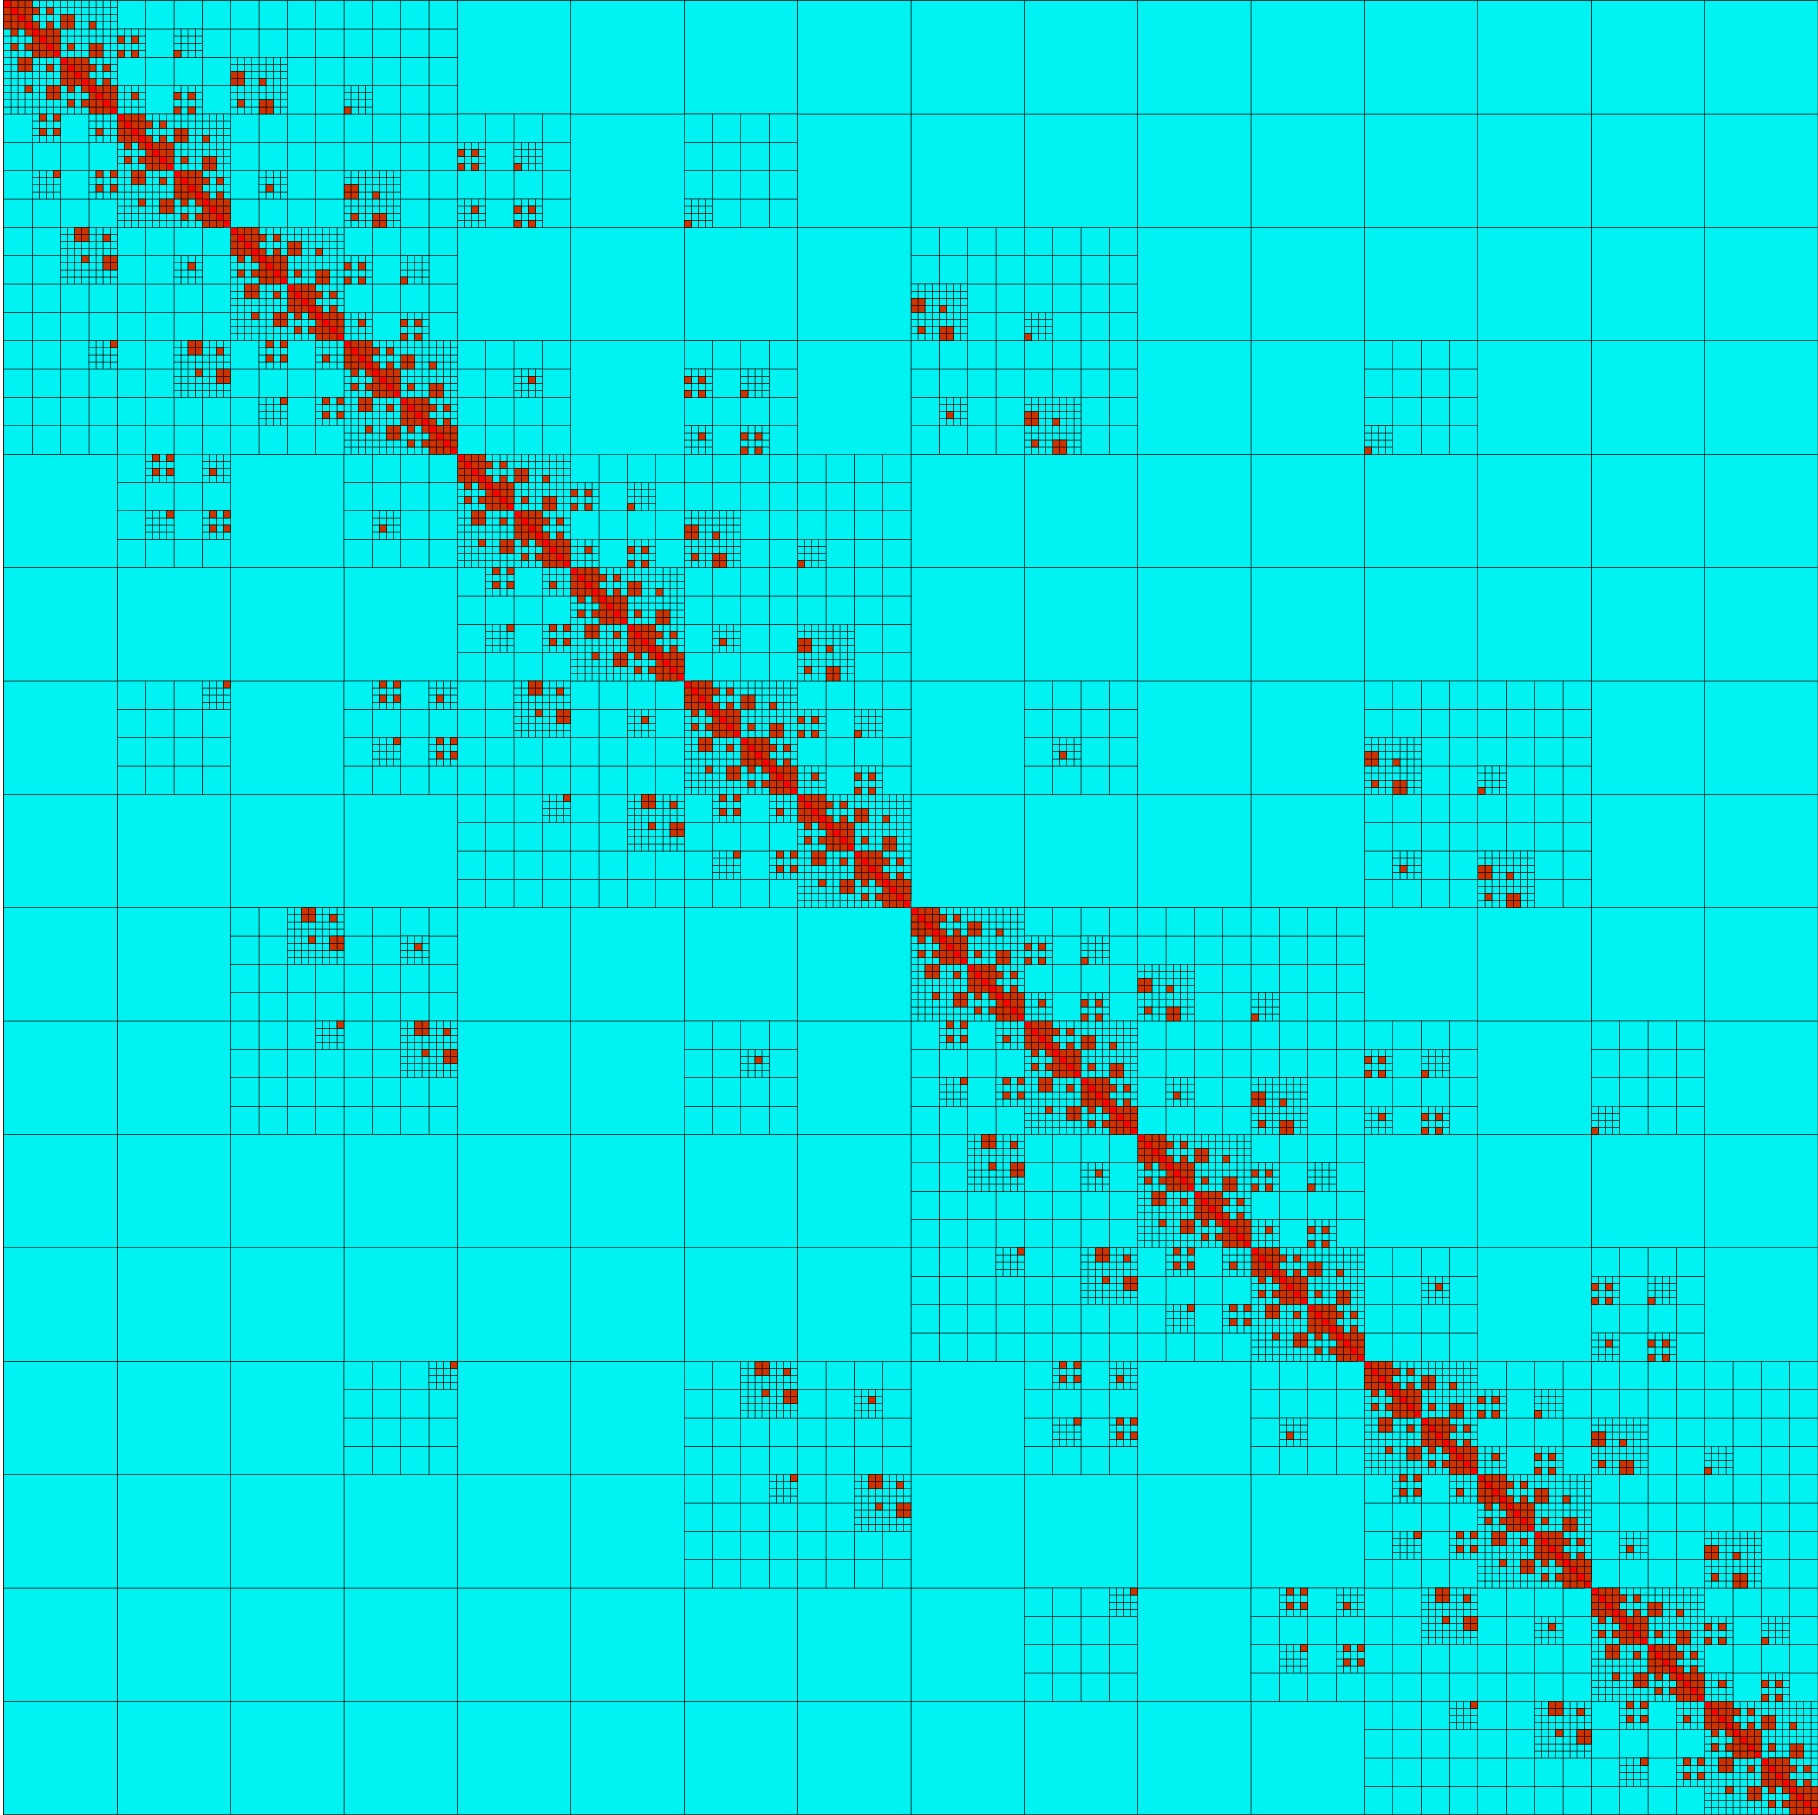
\includegraphics[width=0.5\textwidth]{./images/H2D_level_4.jpg}
	\end{center}
\end{frame}

\begin{frame}{Impact of previous work}
	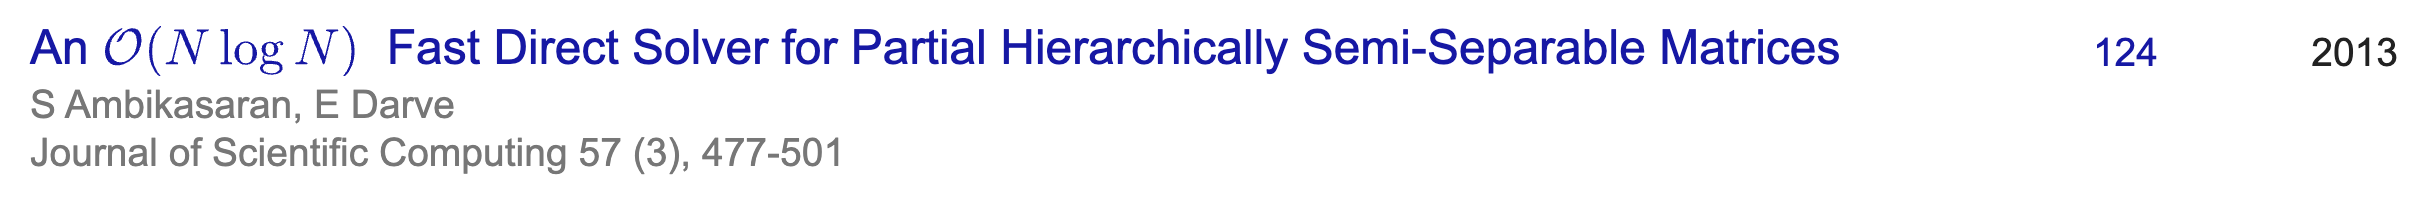
\includegraphics[width=\textwidth]{./images/HODLR_paper.png}\\
	
\includegraphics[width=\textwidth]{./images/HODLR_Code.png}
\end{frame}

\begin{frame}{Impact of previous work}
	\begin{center}
	SIAM LA 2015 Plenary talk\\
	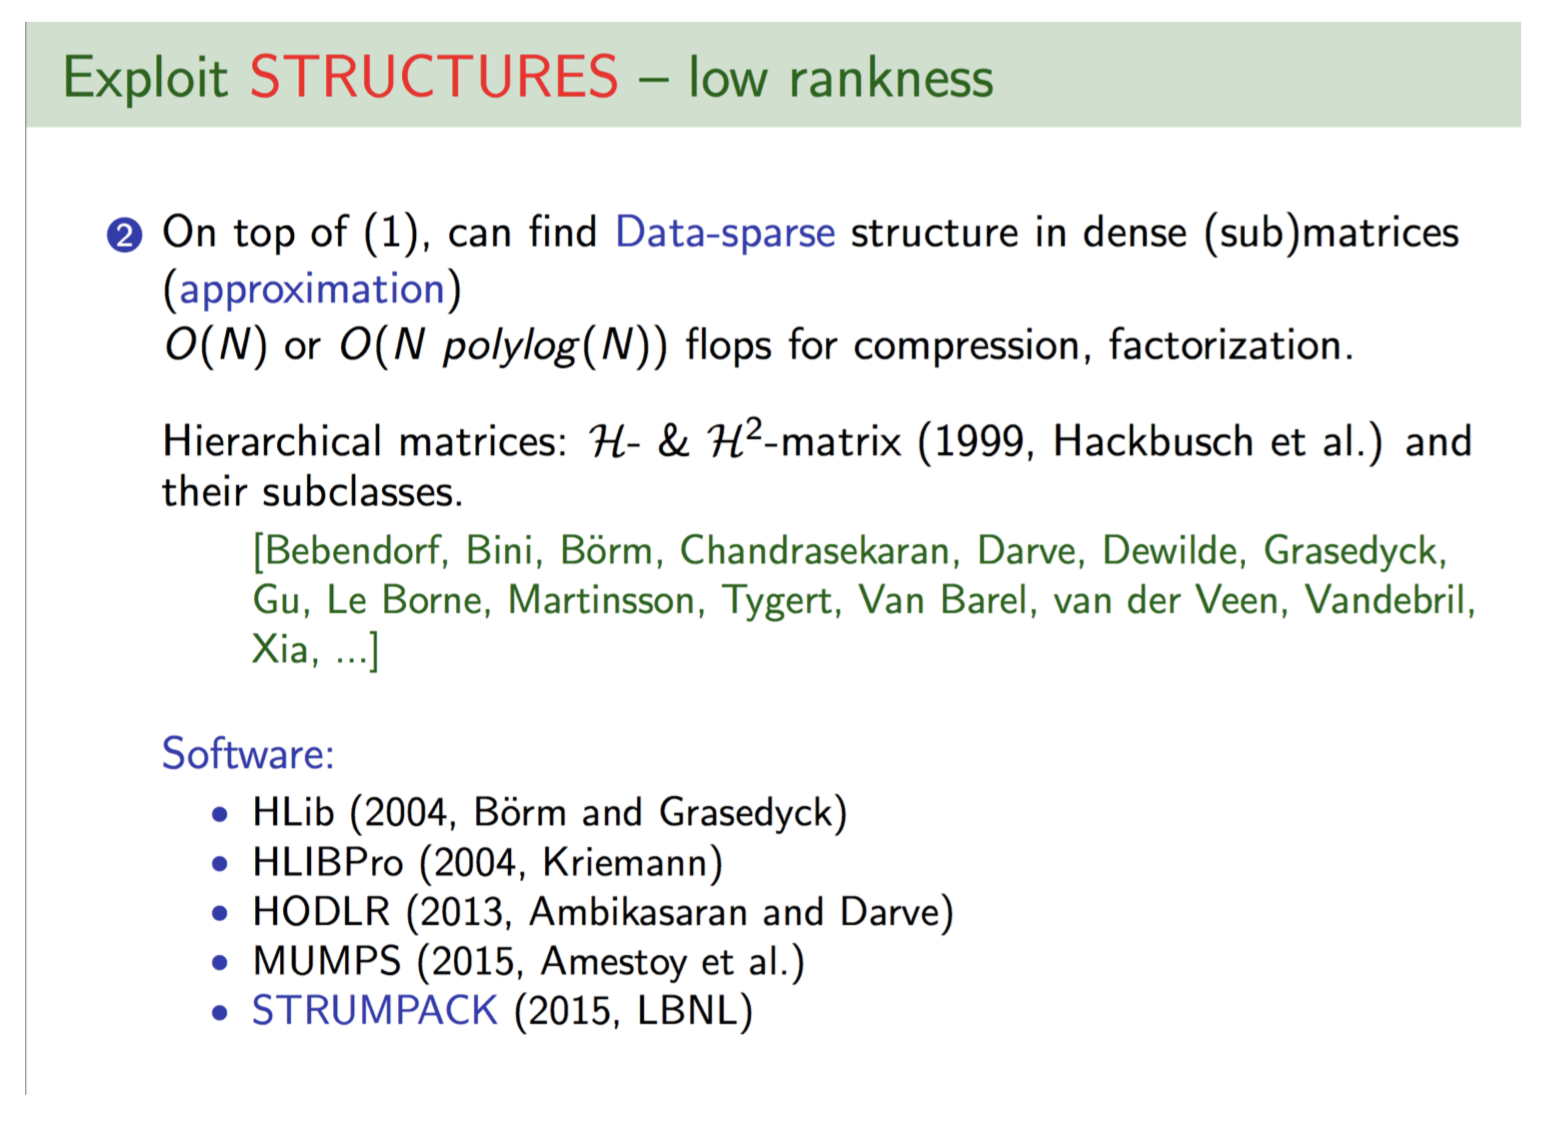
\includegraphics[width=0.5\textwidth]{./images/SIAMLA2015Plenary.png}
	\end{center}
\end{frame}

\begin{frame}{Impact of previous work}
	\begin{center}
	John Von Neumann Lecture at SIAM Annual Meeting 2014\\
	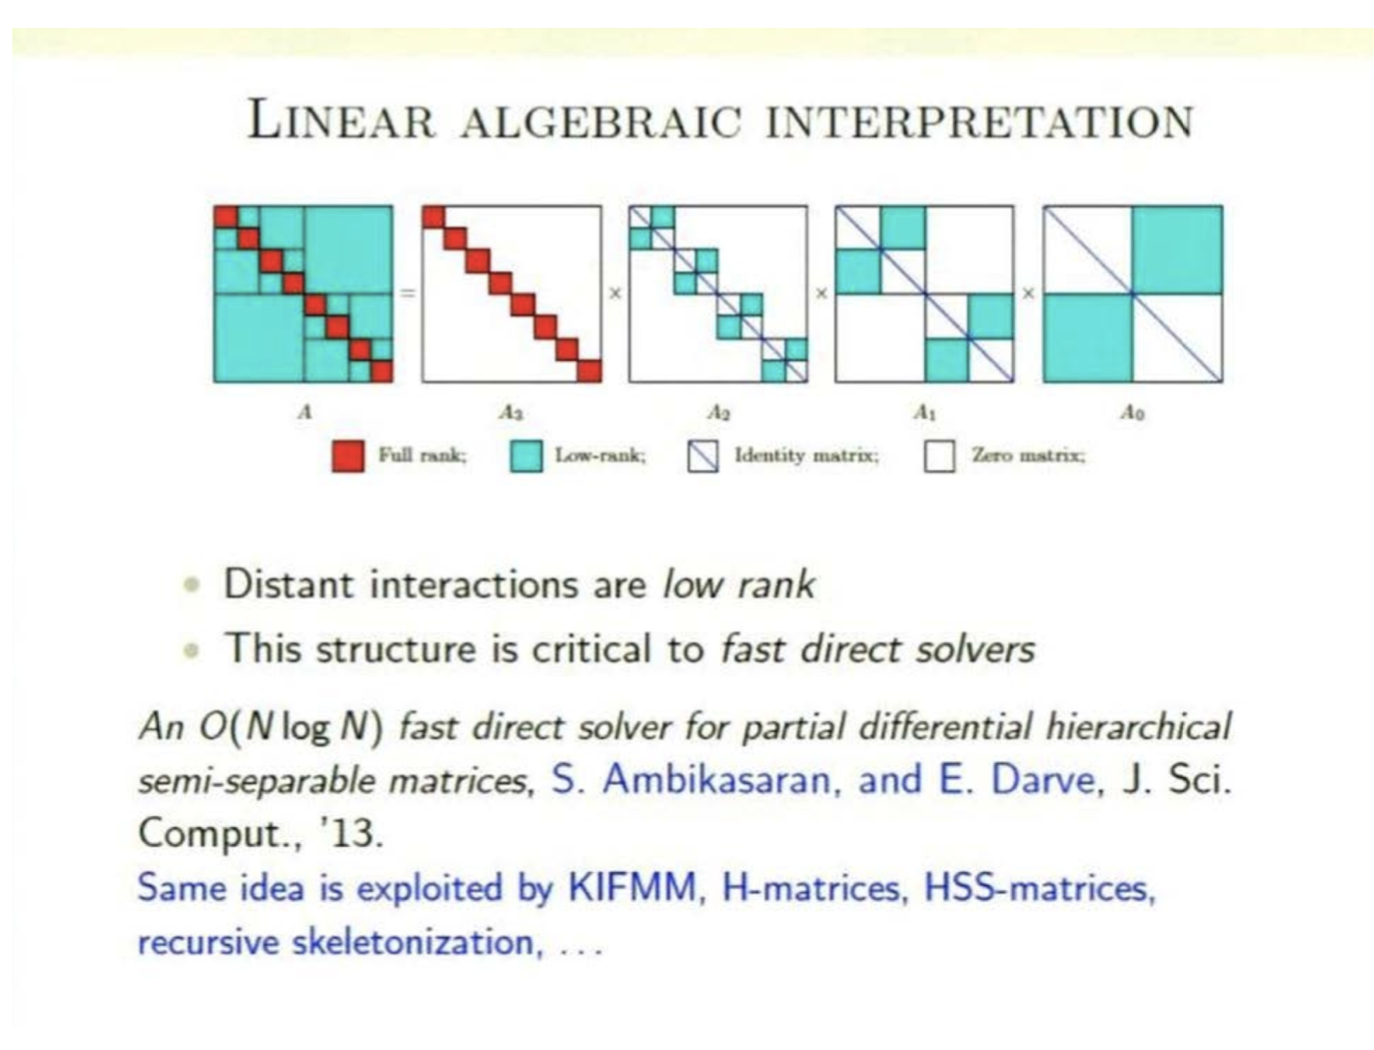
\includegraphics[width=0.5\textwidth]{./images/SIAMVonNeumann2014.png}
	\end{center}
\end{frame}

\begin{frame}{Other high impact work}
	\begin{itemize}
		\item
		George - A fast and flexible library for Gaussian Process Regression\\
		George is now the most preferred solver for performing Gaussian Process Regression.
		\item
		Celerite - A scalable method for Gaussian regression in one dimension
	\end{itemize}
\end{frame}

\begin{frame}{Current Work}
	\begin{itemize}
		\item
		Energy based low-rank factorizations
		\item
		Accelerate Multi-frontal solvers for sparse linear systems
		\item
		High frequency Fast Multipole Method
		\item
		Data driven approaches in combustion
		\item
		Accelerating iterative methods in linear systems
	\end{itemize}
\end{frame}

\end{document}